\documentclass{llncs}  
%\documentclass[runningheads]{llncs}

\usepackage{graphicx} 
\usepackage[T1]{fontenc}
\usepackage{amsmath}
\usepackage[english]{babel}
\usepackage{array,tabularx}
\usepackage{booktabs} 
\usepackage{makeidx}  % allows for index generation
\usepackage{xparse}
\usepackage{moredefs}
\usepackage{lips}
\usepackage{epstopdf} 
% \usepackage{minted}
\usepackage{color}
\usepackage{csquotes}
\usepackage{xcolor}
\usepackage{times}
\usepackage[hidelinks]{hyperref}
\usepackage[nolist,nohyperlinks]{acronym}
\usepackage{comment}
\usepackage{paralist}
\usepackage{cleveref}
\usepackage{wrapfig}
\usepackage{multirow}
\usepackage{microtype}
\usepackage{listings}
\usepackage[super]{nth}

% ------------------
% | WI Adjustments |
% ------------------

% \setlength{\parindent}{0pt} % disable indent globally

\usepackage{float}
% Make table captions above the table
\floatstyle{plaintop}
\restylefloat{table}

%fix captions of figures
\usepackage[style=base,labelfont=bf,labelsep=period,tableposition=top,font=small]{caption}
\captionsetup[figure]{name=Figure}
\setlength{\parskip}{0pt} % no parskip, only parindent
\setlength{\textfloatsep}{18pt plus 0pt minus 18pt} %abstand von text und figure/caption
\setlength{\floatsep}{12pt plus 0pt minus 0pt} %abstand zwischen floats
\setlength{\intextsep}{18pt plus 0pt minus 18pt} %abstand zwischen text und anderen arten von figures

\makeatletter
\renewcommand\@biblabel[1]{#1.}
\makeatother
\addto\captionsenglish{\renewcommand{\bibname}{\leftline{References}}}

% \let\oldbibliography\bibliography% Store \bibliography in \oldbibliography
% \renewcommand{\bibliography}[1]{{%
%  \let\chapter\section% Copy \section over \chapter
%  \oldbibliography{#1}}}% Old \bibliography

% WI footer
\usepackage{fancyhdr}
\fancypagestyle{WI_footer}{\fancyhf{}\renewcommand{\headrulewidth}{0pt}\fancyfoot[L]{\color{black}\scriptsize 17th International Conference on Wirtschaftsinformatik\\February 2022, Nürnberg, Germany}}

\usepackage{cite}

% -----------
% | Custom  |
% -----------
\newcommand{\ks}[1]{\hangindent=0.5cm \textbf{#1}}
\crefformat{footnote}{#2\footnotemark[#1]#3}
% --------------------------
% | Hyphenation in URL env |
% --------------------------
%\usepackage[hyphens]{url}
%\PassOptionsToPackage{hyphens}{url}\usepackage{hyperref}
\expandafter\def\expandafter\UrlBreaks\expandafter{\UrlBreaks%  save the current one
  \do\a\do\b\do\c\do\d\do\e\do\f\do\g\do\h\do\i\do\j%
  \do\k\do\l\do\m\do\n\do\o\do\p\do\q\do\r\do\s\do\t%
  \do\u\do\v\do\w\do\x\do\y\do\z\do\A\do\B\do\C\do\D%
  \do\E\do\F\do\G\do\H\do\I\do\J\do\K\do\L\do\M\do\N%
  \do\O\do\P\do\Q\do\R\do\S\do\T\do\U\do\V\do\W\do\X%
  \do\Y\do\Z}

% ----------------
% | Hyphenation  |
% ----------------
\hyphenation{sus-tain-able}
% ------------------
% | Custom colors  |
% ------------------
% \definecolor{LightGray}{gray}{0.9}
% \definecolor{crowdstrom}{RGB}{46, 170, 225}
% \definecolor{mygreen}{rgb}{0,0.6,0}
% \definecolor{mygray}{rgb}{0.5,0.5,0.5}
% \definecolor{mymauve}{rgb}{0.58,0,0.82}
% \definecolor{mygray}{gray}{0.85}
% \definecolor{mycyan}{rgb}{0.88,1,1}
% \DeclareCaptionFont{white}{\color{white}}
% MaMa Some Useful Column Definitions
\newcolumntype{L}[1]{>{\raggedright\arraybackslash}p{#1}}   % linksbündig mit Breitenangabe
\newcolumntype{C}[1]{>{\centering\arraybackslash}p{#1}}     % zentriert mit Breitenangabe
\newcolumntype{R}[1]{>{\raggedleft\arraybackslash}p{#1}}    % rechtsbündig mit Breitenangabe

% -------------
% | Variables |
% -------------
%\crefformat{footnote}{#2\footnotemark[#1]#3}

% ---------------------------
% | Title page and authors  |
% ---------------------------
\begin{document}
\frontmatter          % for the preliminaries
%\pagestyle{headings}  % switches on printing of running heads

\mainmatter              % start of the contributions


\title{Author Guidelines for the Preparation of Contributions to WI 2022}

%\author{Blinded\inst{1}}
%\authorrunning{Blinded et al.} % abbreviated author list (for running head)
%\institute{Blinded}

\author{First Author\inst{1} \and
Second Author\inst{1} \and
Third Author\inst{1,2} \and
Forth Author\inst{2}}

\institute{Institution, Department, City, Country\\
\email{\{first.author,second.author,third.author\}@example.com} \and
Other Institution, Other Department, Other City, Other Country\\
\email{\{third.author,fourth.author}@anotherexample.com\}}

% -----------------------
% |  Begin of Document  |
% -----------------------
\maketitle
\setcounter{footnote}{0}

% ------------- 
% |  Abstract and Keywords  |
% -------------
\begin{abstract}
The abstract $\{$style \textit{abstract}$\}$ is a mandatory element that should summarize the contents of the paper and contain at least 70 and at most 150 words.\\

{\bfseries Keywords:} Please list your 3-5 keywords {style keywords} here. They should be separated by commas.
\end{abstract}

\thispagestyle{WI_footer}

% ------------- 
% |  Content  |
% -------------

\section{Introduction}
\label{sec:introduction}

You will find the guidelines for the preparation of the International Conference on Wirtschaftsinformatik 2022 (WI 2022) proceedings here. 
Your contribution has to be prepared by using this Microsoft Word template. 
In essence, we ask you to make your paper look exactly like this document. 
The easiest way to do this is by simply replacing the content with your own material.

\section{Preparation of Your Paper}
\label{sec:theoretical_background}
\subsection{How to Start Writing a New Document Using the Template}
\begin{enumerate}
    \item Save this document and start writing your paper. Edit the template instead of creating a new document that is based on the template.
    \item The revised submission starts directly after the keywords on the cover page.
\end{enumerate}

\subsection{Structuring Your Paper}
\subsubsection{Affiliations.} The affiliated institutions \{\verb|\institutions{}|\} have to be listed directly below the names of the authors \{\verb|\author{}|; authors seperated by \verb|\and|\}. 
No academic titles or descriptions of academic positions should be included in the addresses. 
This information should either be omitted altogether (preferably), or it should be included in a footnote at the end of the first page (to sign remarks pertaining to the title or the authors’ names, symbols should be used (e.g., “*”) instead of a number). 
Multiple affiliations should be marked with superscript Arabic numerals, and they should each start on a new line as shown in this document. 
In addition to the name of your affiliation, we would ask you to give the town and the country in which it is situated. 
If you prefer to include the entire postal address, then please feel free to do so. 
Email addresses should start on a new line and be grouped per affiliation.

\subsubsection{Headings.} 
Headings should be capitalized (i.e., all words except articles, prepositions, and conjunctions should be set with an initial capital letter). 
Hyphenated words are subject to a special rule. 
If the first word can stand alone, the second word should be capitalized. 
Here are some examples of headings: “Criteria to Disprove Context-Freeness of Collage Languages”, “A User-Friendly and Extendable Data Distribution System”, “Multi-flip Networks: Parallelizing GenSAT”. 
Headings should, with the exception of the title {style papertitle}, be aligned to the left. 
Only the first two levels of section headings should be numbered, as shown in Table 1 (this should be done automatically). 
The heading of the reference section with a \nth{1}-level heading and without a numeration is an exception. 
The respective font sizes are also given in Table 1. Kindly refrain from using “0” when numbering your headings.

\begin{table}[htb]
\centering
\caption{Font sizes of headings $\{$style table caption$\}$}
\label{tab:my-table}
\begin{tabular}{@{}lll@{}}
\toprule
\textit{Heading level} & \textit{Example} & \textit{Font size and style} \\ \midrule
Title (centered) & \Large{A Paper Title} & 14 point, bold \\
1st-level heading & \large{1 Introduction} & 12 point, bold \\
2nd-level heading & \textbf{2.1 Printing Area} & 10 point, bold \\
3rd-level heading & \textbf{Run-in Heading in Bold.} Text follows & 10 point, bold\\
4th-level heading & \textit{Lowest Level Heading.} Text follows & 10 point, italic \\ \bottomrule
\end{tabular}
\end{table}

\subsubsection{Tables.} 
You should use normal text {style normal text} for the contents of any table. 
Tables covering more than one page are to be avoided. 
If you absolutely have to include a table covering more than one page, make sure that the table heading is repeated on every page. 
Tables are to be numbered and captions should always be positioned above the tables.

\subsubsection{Normal Text.}
You should use normal text (Times New Roman, font size 10) for the first paragraph in a chapter, after figures, tables, listings, and formulas (without indentation), as well as for all following paragraphs within a chapter. 
Following paragraphs will be indented automatically.

\subsubsection{Lemmas, Propositions, and Theorems.}
The numbers assigned to lemmas, propositions, and theorems, etc. should appear in consecutive order, starting with Lemma 1. 
Please do not include section counters in the numbering such as “Theorem 1.1”.

\subsection{Figures} 
It is essential that all illustrations are as clear and as legible as possible. 
Vector graphics – instead of rasterized images – should be used for diagrams and schemas whenever possible. 
Please check that the lines in line drawings are not interrupted and have a constant width. 
Grids and details within the figures must be clearly legible and may not be written on top of each other. 
The lettering in figures and tables should not use font sizes smaller than 6 pt ($\sim$ 2 mm character height). 
Figures are to be numbered and to have a caption that should always be positioned under the figures.

\begin{figure}[htp]
    \centering
    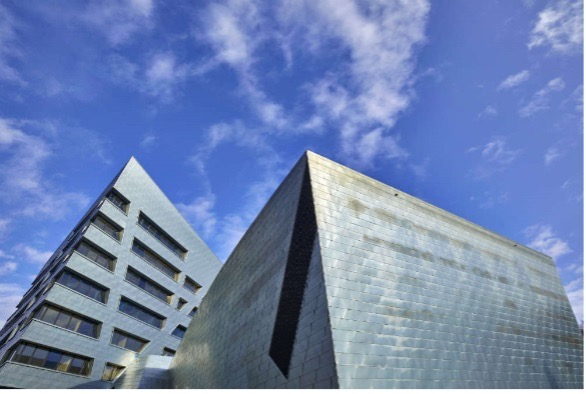
\includegraphics[width=0.65\textwidth]{figures/image.JPG}
    \caption{Picture}
    \label{fig:my_label}
\end{figure}

Captions have to be set in 9-point type. If they are short, they have to be centered between the margins (Fig. \ref{fig:my_label} shows an example). Longer captions covering more than one line have to be justified. Captions that do not constitute a full sentence do not have a period.

Text fragments of fewer than four lines should not appear at the top or bottom of a page and should not follow a table or figure. In such cases, setting the figures right at the top or right at the bottom of the page is better. A figure should never be placed in the middle of a paragraph.

\subsection{Formulas}
Displayed equations or formulas have to be centered and set on a separate line (with an extra line or half line space above and below). Displayed expressions should be numbered for reference. The numbers should be consecutive within the contribution, with numbers enclosed in parentheses and set on the right margin. Please do not include section counters in the numbering.

\begin{equation}
    x + y = z
\end{equation}

\subsection{Footnotes}

The superscript numeral used to refer to a footnote has to appear in the text either directly after the word to be discussed or – in relation to a phrase or a sentence – following the punctuation mark (comma, semicolon, or period)\footnote{The footnote numeral is left-justified and the text follows with the usual word spacing }.  
Please note that no footnotes may be included in the abstract.

\subsection{Program Code}
Program listings or program commands in the text are normally set in typewriter font: 

\begin{lstlisting}
#include<stdio.h>

    int main() {
	printf("Hello World\n");
	return 0;
}
\end{lstlisting}

\subsection{Other Styles}
Besides the styles mentioned above, there are more usable format specifications:
\begin{itemize}
    \item[•] Listings
    \item[•] Numeration
    \item[•] Reference 
\end{itemize}

\subsection{Citations and Bibliography}
Authors using software tools for managing bibliographies (such as Endnote, Citavi, Mendeley) can apply the preconfigured style format Lecture Notes in Computer Science.

For citations of tables and figures in the text, you have to use square brackets and consecutive numbers. 
Numbers should be grouped where appropriate. 
Write \cite{smith1981identification,may2006zib,foster1999grid,czajkowski2001grid,foster2002physiology} 
but \cite{smith1981identification}, \cite{foster1999grid}, \cite{foster2002physiology}, etc. 
The numbers in the bibliography section have to be without square brackets. 

References should be published materials accessible to the public. 
Internal technical reports may be cited only if they are easily accessible (i.e., you can provide the address to obtain the report within your citation) and may be obtained by any reader. 
Private communications should be acknowledged (e.g., with a footnote), not referenced. 
Please base your references on the examples given in the reference section of this instruction and write all references using the Latin alphabet.
If the title of the book you are referring to is, for example, in Russian or Chinese, then please write (in Russian) or (in Chinese) at the end of the transcript or translation of the title. 
Word may try to automatically ‘underline’ hotlinks in your references; the correct style is NO underlining. 
Please make sure that all your sources are correctly listed in the reference section.

The reference section at the end of this paper shows a sample reference list with entries for journal articles \cite{smith1981identification}, 
a book chapter \cite{may2006zib}, 
a book \cite{foster1999grid}, 
proceedings without editors \cite{czajkowski2001grid}, 
technical reports \cite{foster2002physiology}, 
as well as URLs \cite{ncb}. 

\section{Acknowledgements}
You can add your acknowledgements to the revised paper. Acknowledgements are added before the references.

% ----------------
% | Bibliography |
% ----------------

\bibliographystyle{splncs04}
\bibliography{./literature.bib}
% ---------------------
% |  End of Document  |
% ---------------------

\end{document}